\documentclass{beamer}\usepackage[]{graphicx}\usepackage[]{color}
%% maxwidth is the original width if it is less than linewidth
%% otherwise use linewidth (to make sure the graphics do not exceed the margin)
\makeatletter
\def\maxwidth{ %
  \ifdim\Gin@nat@width>\linewidth
    \linewidth
  \else
    \Gin@nat@width
  \fi
}
\makeatother

\definecolor{fgcolor}{rgb}{0.345, 0.345, 0.345}
\newcommand{\hlnum}[1]{\textcolor[rgb]{0.686,0.059,0.569}{#1}}%
\newcommand{\hlstr}[1]{\textcolor[rgb]{0.192,0.494,0.8}{#1}}%
\newcommand{\hlcom}[1]{\textcolor[rgb]{0.678,0.584,0.686}{\textit{#1}}}%
\newcommand{\hlopt}[1]{\textcolor[rgb]{0,0,0}{#1}}%
\newcommand{\hlstd}[1]{\textcolor[rgb]{0.345,0.345,0.345}{#1}}%
\newcommand{\hlkwa}[1]{\textcolor[rgb]{0.161,0.373,0.58}{\textbf{#1}}}%
\newcommand{\hlkwb}[1]{\textcolor[rgb]{0.69,0.353,0.396}{#1}}%
\newcommand{\hlkwc}[1]{\textcolor[rgb]{0.333,0.667,0.333}{#1}}%
\newcommand{\hlkwd}[1]{\textcolor[rgb]{0.737,0.353,0.396}{\textbf{#1}}}%
\let\hlipl\hlkwb

\usepackage{framed}
\makeatletter
\newenvironment{kframe}{%
 \def\at@end@of@kframe{}%
 \ifinner\ifhmode%
  \def\at@end@of@kframe{\end{minipage}}%
  \begin{minipage}{\columnwidth}%
 \fi\fi%
 \def\FrameCommand##1{\hskip\@totalleftmargin \hskip-\fboxsep
 \colorbox{shadecolor}{##1}\hskip-\fboxsep
     % There is no \\@totalrightmargin, so:
     \hskip-\linewidth \hskip-\@totalleftmargin \hskip\columnwidth}%
 \MakeFramed {\advance\hsize-\width
   \@totalleftmargin\z@ \linewidth\hsize
   \@setminipage}}%
 {\par\unskip\endMakeFramed%
 \at@end@of@kframe}
\makeatother

\definecolor{shadecolor}{rgb}{.97, .97, .97}
\definecolor{messagecolor}{rgb}{0, 0, 0}
\definecolor{warningcolor}{rgb}{1, 0, 1}
\definecolor{errorcolor}{rgb}{1, 0, 0}
\newenvironment{knitrout}{}{} % an empty environment to be redefined in TeX

\usepackage{alltt}

\def\currentCourse{An introduction to graph analysis and modeling}
\def\currentInstitute{MSc in Statistics for Smart Data -- ENSAI}
\def\currentLogo{logo_ensai}
\def\currentDate{Automn semester, 2017}
\def\currentChapter{Topology Inference}

\definecolor{genecolor}{RGB}{94,135,173}


% THEME BEAMER

\usetheme{teaching}
\usefonttheme[onlymath]{serif}
\graphicspath{{figures/}}
\usepackage[ruled,vlined,linesnumbered]{algorithm2e}
\usepackage{tikz}
\usetikzlibrary{calc,shapes,backgrounds,arrows,automata,shadows,positioning}
\tikzstyle{every state}=[fill=red,draw=none,scale=0.7,font=\small,text=white]
\tikzstyle{every edge}=[-,shorten >=1pt,auto,thin,draw]
\tikzstyle{alertstate}=[fill=bleu]
\definecolor{genecolor}{RGB}{94,135,173}

\title{\currentCourse}

\subtitle{\huge\currentChapter\normalsize}

\institute{\currentInstitute}

\date{Autumn semester 2017}



\AtBeginSection{
  \begin{frame}<beamer>
    \frametitle{Outline}
    \framesubtitle{\insertpart}
    \tableofcontents[currentsection,currentsubsection, subsectionstyle=show/shaded/hide]  
  \end{frame}
}

\AtBeginSubsection{
  \begin{frame}<beamer>
    \frametitle{Outline}
    \framesubtitle{\insertpart}
    \tableofcontents[currentsection,currentsubsection, subsectionstyle=show/shaded/hide]  
  \end{frame}
}

\AtBeginSubsubsection{
  \begin{frame}<beamer>
    \frametitle{Outline}
    \framesubtitle{\insertpart}
    \tableofcontents[currentsection,currentsubsection, subsectionstyle=show/shaded/hide]  
  \end{frame}
}

\newcommand{\dotitlepage}{%
  \begin{frame}
    \titlepage
    \vfill
    \begin{center}
        \scriptsize\url{http://julien.cremeriefamily.info}
    \end{center}
    \vfill
    \includegraphics[width=1.5cm]{\currentLogo}\hfill
    
\includegraphics[width=2.5cm]{logo_inra}
  \end{frame}
  %
}

\newcommand{\dotoc}{%
  \begin{frame}
    \frametitle{Outline}
    \tableofcontents[currentsection,
    sectionstyle=show/show,
    subsectionstyle=hide]
  \end{frame}
  %
}



\usetikzlibrary{calc,shapes,backgrounds,arrows,automata,shadows,positioning}
\tikzstyle{every state}=[fill=red,draw=none,scale=0.7,font=\small,text=white]
\tikzstyle{every edge}=[-,shorten >=1pt,auto,thin,draw]
\tikzstyle{alertstate}=[fill=mblue]

\pgfdeclareimage[width=.18\textwidth]{microarray}{figures/puce}
\pgfdeclareimage[width=.3\textwidth]{affymetrix}{figures/affy}

\pgfdeclareimage[width=.18\textwidth]{sequencer}{figures/sequencer}
\pgfdeclareimage[width=.25\textwidth]{ngs}{figures/ngs_data}

\pgfdeclareimage[width=.2\textwidth]{rna_seq}{figures/rna_seq}
\pgfdeclareimage[width=.5cm]{computer}{figures/computer}
\IfFileExists{upquote.sty}{\usepackage{upquote}}{}
\begin{document}

\dotitlepage

\begin{frame}
  \frametitle{Introduction}

  \begin{block}{first two courses: \alert{Analysis of an existing, observed network}}
    \vspace{-.25cm}  
    \begin{itemize}
      \item[$\rightsquigarrow$] \alert{basic characterization}
      \item[$\rightsquigarrow$] \alert{find an underlying organization} (clustering)
    \end{itemize}
  \end{block}

  \begin{block}{Today: \alert{reconstruct (infer) a network from external data}}<2->
    Become familiar with
    \begin{itemize}
      \item Gaussian graphical models,
      \item sparse inference methods ($\ell_1$-regularization \textit{a.k.a} the \alert{Lasso}).
    \end{itemize}
  \end{block}

  \begin{block}{Canonical example: \alert{Genomic data}}<3->
    We consider examples from life science, but everything said extends to
    \begin{itemize}
      \item Sociology, Astrophysics, Stock exchange, Insurance data, \dots
      \item \dots any multivariate data. 
    \end{itemize}
  \end{block}

\end{frame}

\begin{frame}
  \frametitle{Omic: parallel measurement of \alert{many} biological features}

  Focus e.g. on \textit{transcription},    looking toward \textcolor{genecolor}{\textit{gene regulatory networks}}

  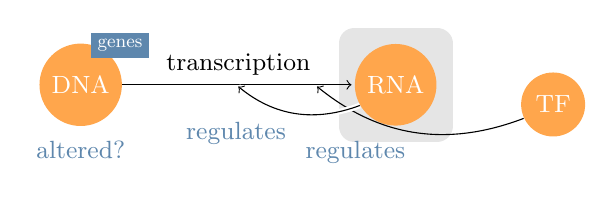
\begin{tikzpicture}
    \begin{small}
      \tikzstyle{every state}=[fill=orange!70!white,draw=none,text=white]
      \node[state] (dna) at (0,0) {DNA};
      \node[state] (rna) at (4,0) {RNA};
      \node[state] (tf) at (6,-0.25) {TF};
      \node[draw=none,text=white,fill=genecolor, scale=0.75] (gene) at (0.5,0.5) {genes};
      \node[draw=none,text=genecolor,fill=white] (alter) at ($(dna.south) -(0,3mm)$) {altered?};

      \path
      (dna) edge [->] node[above] {\alert{transcription}} (rna)
      (tf) edge [bend left, ->] node[midway] {\textcolor{genecolor}{regulates}} ($(rna.west) -(5mm,0)$)
      (rna) edge [-,line width=2pt,draw=white,bend left] ($(rna.west) -(15mm,0)$)
      (rna) edge [bend left, ->] node {\textcolor{genecolor}{regulates}} ($(rna.west) -(15mm,0)$);
    \end{small}

    \begin{pgfonlayer}{background}
      \filldraw [line width=4mm,join=round,black!10]
      (rna.north -| rna.west) rectangle (rna.south -| rna.east);
    \end{pgfonlayer}

  \end{tikzpicture}

  \only<1>{
    \begin{tikzpicture}
      \node at (0,-.25) {\pgfuseimage{affymetrix}};
      \node[fill=mred, text=white,single arrow]
      (sig) at (3.5,-.25) {\sf \scriptsize signal processing};
      \node[opacity=.75] (array1) at (7.25,0.25) {\pgfuseimage{microarray}};
      \node[opacity=.9] (array2) at (7.5,0) {\pgfuseimage{microarray}};
      \node[opacity=.95] (array3) at (7.75,-0.25) {\pgfuseimage{microarray}};
      \node at (8,-0.5) (array4) {\pgfuseimage{microarray}};

      \begin{pgfonlayer}{background}
        \filldraw [line width=4mm,join=round,black!10]
        (array1.north -| array1.west) rectangle (array4.south -| array4.east);
      \end{pgfonlayer}

      \node at (7,-3) {%
        $\mathbf{X} = \begin{pmatrix}
          x_1^1 & x_1^2 & x_1^3 & \dots & x_1^p \\
          \vdots \\
          x_n^1 & x_n^2 & x_1^2 & \dots & x_n^p \\
        \end{pmatrix}$};

      \node (output) at (0,-3) {
        \begin{tabular}{@{}l@{}}
          \small Matrix of features $n\ll p$\\ \hline
          \scriptsize Expression levels of $p$ \\
          \scriptsize probes are simultaneously \\
          \scriptsize monitored for $n$ individuals
        \end{tabular}
      };

      \begin{pgfonlayer}{background}
        \filldraw [line width=4mm,join=round,black!10]
        (output.north -| output.west) rectangle (output.south -| output.east);
      \end{pgfonlayer}

      \node[fill=mred, text=white,single arrow, shape border rotate =180]
      (inference) at (3.35,-3) {\sf \scriptsize pretreatment};
    \end{tikzpicture}
  }

  \only<2>{
    \begin{tikzpicture}
      \node at (0,-.25) {\pgfuseimage{sequencer}};

      \node[fill=mred, text=white,single arrow]
      (sig) at (3.5,-.25) {\sf \scriptsize assembling};

      \node[opacity=.75] (array1) at (7.25,0.25) {\pgfuseimage{ngs}};
      \node[opacity=.9] (array2) at (7.5,0) {\pgfuseimage{ngs}};

      \begin{pgfonlayer}{background}
        \filldraw [line width=4mm,join=round,black!10]
        (array1.north -| array1.west) rectangle (array2.south -| array2.east);
      \end{pgfonlayer}

      \node at (7,-2.75) {%
        $\mathbf{X} = \begin{pmatrix}
          k_1^1 & k_1^2 & k_1^3 & \dots & k_1^p \\
          \vdots \\
         k_n^1 & k_n^2 & k_1^2 & \dots & k_n^p \\
        \end{pmatrix}$};

      \node (output) at (0,-2.75) {
        \begin{tabular}{@{}l@{}}
          \small Matrix of features $n\lll p$\\ \hline
          \scriptsize Expression counts are extracted \\
          \scriptsize from small repeated sequences \\
          \scriptsize and monitored for $n$ individuals
        \end{tabular}
      };

      \begin{pgfonlayer}{background}
        \filldraw [line width=4mm,join=round,black!10]
        (output.north -| output.west) rectangle (output.south -| output.east);
      \end{pgfonlayer}

      \node[fill=mred, text=white,single arrow, shape border rotate =180]
      (inference) at (3.35,-2.75) {\sf \scriptsize pretreatment};
    \end{tikzpicture}
    }
\end{frame}

\begin{frame}
  \frametitle{Network inference: a challenging problem}

  \begin{columns}[c]
    \begin{column}{.55\textwidth}
      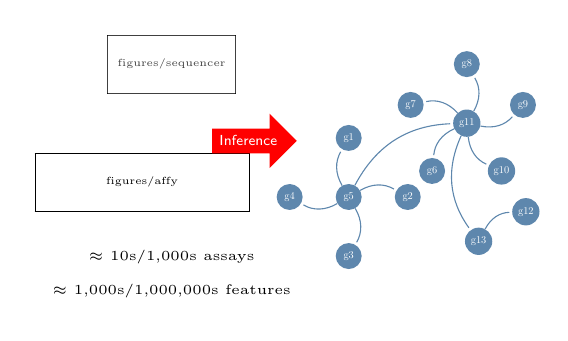
\begin{tikzpicture}[scale=0.75]
        \node[scale=0.75,opacity=0.75] at (-3,3) {\pgfuseimage{sequencer}};
        \node[scale=0.75] at (-3.5,1) {\pgfuseimage{affymetrix}};
        \node[scale=0.75,fill=red, text=white,single arrow]
        (inference) at (-1.7,1.7) {\sf \scriptsize Inference};

        \node at (-3,-0.5) {\begin{tabular}{@{}c@{}}
            \tiny $\approx$ 10s/1,000s assays \\
            \tiny $\approx $ 1,000s/1,000,000s features \\
          \end{tabular}
        };

        %% UN GRAPH
        \tikzstyle{every edge}=[-,>=stealth',shorten >=1pt,auto,thin,draw,color=genecolor]
        \tikzstyle{every node}=[fill=genecolor]
        \tikzstyle{every state}=[draw=none,text=white,scale=0.5, transform shape]

        % premier cluster
        \node[state] (A1) at (0,1.75) {g1};
        \node[state] (A2) at (1,0.75) {g2};
        \node[state] (A3) at (0,-.25) {g3};
        \node[state] (A4) at (-1,0.75) {g4};
        \node[state] (A5) at (0,0.75) {g5};

        \foreach   \name/\angle/\text   in  {B1/234/g6,   B2/162/g7,
          B3/90/g8, B4/18/g9, B5/-54/g10} {
          \node[state,xshift=4cm,yshift=4cm]     (\name)    at
          (\angle:1cm) {\text}; }

        \node[state] (B6) at (2,2) {g11};
        \node[state] (C1) at (3,0.5) {g12};
        \node[state] (C2) at (2.2,0) {g13};

        \path
        (A5) edge [bend left] (A1)
        (A5) edge [bend left] (A2)
        (A5) edge [bend left] (A3)
        (A5) edge [bend left] (A4)
        (B6) edge [bend right] (B1)
        (B6) edge [bend right] (B2)
        (B6) edge [bend right] (B3)
        (B6) edge [bend right] (B4)
        (B6) edge [bend right] (B5)
        (C2) edge [bend left] (C1)
        (A5) edge [bend left] (B6)
        (B6) edge [bend right] (C2);
      \end{tikzpicture}
    \end{column}
    \begin{column}{.45\textwidth}
      \begin{footnotesize}
        \begin{enumerate}
        \item Nodes are fixed
            \noindent\begin{itemize}
            \item \scriptsize \alert{restricted}   to  a   set  of   interest
            \end{itemize}
        \item Edges (interactions) are inferred
          \begin{scriptsize}
            \begin{itemize}
            \item \scriptsize based upon \alert{statistical} concepts
            \end{itemize}
          \end{scriptsize}
        \end{enumerate}
      \end{footnotesize}
    \end{column}
  \end{columns}

  \begin{block}{Statistical question}
    \vspace{-.25cm}
    \begin{enumerate}
    \item Variable selection (which edges?)
    \end{enumerate}
  \end{block}

  \begin{block}{Main statistical challenges}
    \vspace{-.25cm}
    \begin{enumerate}
    \item (Ultra) High dimensionality ($n<p$, $n\lll p$)
    \item Heterogeneity/structure of the data
    \end{enumerate}
  \end{block}

\end{frame}



\begin{frame}
  \frametitle{Outline}
  \tableofcontents
\end{frame}

\section{Network and data modeling}

\begin{frame}
  \frametitle{References}

    \begin{thebibliography}{99}
      \setbeamertemplate{bibliography item}[book]

    \bibitem[JW]{JW} Graphical Models in Applied Multivariate Statistics, \textcolor{black}{Joe Whittaker}
    \bibitem[SL]{SL} Graphical Models, \textcolor{black}{S. Lauritzen}
    \end{thebibliography}

\end{frame}

\subsection{Statistical dependence}

\begin{frame}
  \frametitle{Modeling relationship between variables}
  \framesubtitle{Independence}

  \begin{definition}[Independence of events]
    Two events $A$ and $B$ are independent if and only if
    \begin{equation*}
      \prob(A,B) = \prob(A) \prob(B),
    \end{equation*}
    which is usually denoted by $A \indep B$. Equivalently,
    \begin{itemize}
    \item $A \indep B \Leftrightarrow \prob(A | B) = \prob(A)$,
    \item $A \indep B \Leftrightarrow \prob(A | B) = \prob(A | B^c) $
    \end{itemize}
  \end{definition}

  \begin{example}[class vs party]<2>
    \vspace{-.5cm}
    \begin{table}
      \centering
      \begin{small}
      \begin{tabular}{cc}
        \begin{tabular}{rrr}
        & \multicolumn{2}{c}{party} \\
        class & Labour & Tory \\ \hline
        working & 0.42 & 0.28 \\
        bourgeoisie & 0.06 & 0.24 \\
      \end{tabular} 
      & 
      \begin{tabular}{rrr}
        & \multicolumn{2}{c}{party} \\
        class & Labour & Tory \\ \hline
        working & 0.60 & 0.40 \\
        bourgeoisie & 0.20 & 0.80 \\
      \end{tabular} 
      \end{tabular} 
      \caption{Joint probability (left) vs. conditional probability (right)} 
      \end{small}
    \end{table}
  \end{example}
\end{frame}

\begin{frame}
  \frametitle{Limits of correlation for network reconstruction}
  
  \includegraphics<1>[width=.65\textwidth]{cor_plot}

  \includegraphics<2>[width=.65\textwidth]{pcor_plot}
  
\end{frame}

\begin{frame}
  \frametitle{Modeling relationships between variables (2)}
  \framesubtitle{Conditional independence}
  
  Generalizing  to more  than two  events requires  strong assumptions
  (mutual independence). Better handle with

  \begin{definition}[Conditional independence of events]
    Two events $A$ and $B$ are conditionally independent if and only if
    \begin{equation*}
      \prob(A,B | C) = \prob(A|C) \prob(B|C),
    \end{equation*}
    which is usually denoted by $A \indep B | C$ 
  \end{definition}

  \begin{example}[Does QI depends on weight?]
    Consider  the  events $A  =  "\text{having low  QI}"$,  $B  = \text{"having  low
    weight"}$. \only<3>{Estimating\footnote{stupidly}  $\prob(A,B)$,  $\prob(A)$  and
    $\prob(B)$ in a sample would lead to
    \begin{equation*}
      \prob(A,B) \neq \prob(A) \prob(B)
    \end{equation*}}
  \only<4>{But in fact, introducing $C = \text{"having a given age"}$,
    \begin{equation*}
      \prob(A,B|C) = \prob(A|C) \prob(B|C)
    \end{equation*}}
\end{example}
  
\end{frame}

\begin{frame}
  \frametitle{(Conditional) independence of random vectors}
  \framesubtitle{A ``natural'' generalization}

   \begin{definition}   Consider   3   random   variables   $X,Y,Z$   with
     distribution $f_X,f_Y,f_Z$, jointly $f_{XY}, f_{XYZ}$. Then,
     \begin{itemize}
     \item  $X$  and $Y$  are  independent  iif  $f_{XY}(x,y) =  f_{X}(x)
       f_{Y}(y)$;
     \item $X$ and $Y$ are conditionally independent on $Z$, $z:f_Z(z)>0$ iif
       $f_{XY|Z}(x,y;z) = f_{X|Z}(x;z) f_{Y|Z}(y;z)$.
     \end{itemize}
   \end{definition}


   \def\firstcircle{(0,0) circle (2.25cm)}
   \def\secondcircle{(45:3.5cm) circle (2.25cm)}
   \def\thirdcircle{(0:3.5cm) circle (2.25cm)}

   % Now we can draw the sets:
   \begin{figure}[htbp!]
     \centering
     \begin{tikzpicture}[scale=.5]
     \draw \firstcircle node[left= -.25cm] {$f; X\indep Z | Y$};
     \draw \secondcircle node [above=.5cm] {$f; X\indep Y | Z$};
     \draw \thirdcircle node [right=-.25cm] {$f; Y\indep Z | X$};
     \draw (-2,3) node {$f; f_{XYZ}$};
     \draw (2.1,1) node {$f; f_{X} f_{Y} f_{Z}$};
   \end{tikzpicture}
     \caption{Mutual independence, Conditional dependence, full dependence.}
   \end{figure}

 \end{frame}

\subsection{Gaussian Graphical models}

\begin{frame}
  \frametitle{Graphical models}
  \begin{block}{Definition}
    A graphical model gives  a graphical (intuitive) representation of
    the dependence structure of a probability distribution, by linking
    
    \begin{enumerate}
    \item a random  vector (or a set of random  variables.)  $X = \{X_1,
      \dots, X_p\}$ with distribution $\prob$, \bigskip
    \item a graph $\mathcal{G} = (\mathcal{P}, \mathcal{E})$ where
      \begin{itemize}
      \item $\mathcal{P}=\{1,\dots,p\}$ is  the set of nodes associated
        to each variable,
      \item $\mathcal{E}$ is a  set of edges describing the dependence
        relationship of $X\sim \prob$.
      \end{itemize}
    \end{enumerate}
   \end{block}

   \vfill

  \begin{definition}<2> The  \alert{conditional independence graph}  of a
    random vector  $X$ is the \alert{undirected}  graph $\mathcal{G} =
    \{\mathcal{P},    \mathcal{E}\}$   with    the    set   of    node
    $\mathcal{P}=\{1,\dots,p\}$ and where
    \begin{equation*}
      (i,j) \notin \mathcal{E} \Leftrightarrow X_i \indep X_j | \mathcal{P} \backslash
      \{i,j\}.
    \end{equation*}
  \end{definition}

\end{frame}

\begin{frame}
  \frametitle{Conditional Independence Graphs}
  \framesubtitle{An example}
  
  Let  $X_1,  X_2, X_3,  X_4$  be  four  random variables  with  joint
  probability density  function $f_X(x) =  \exp(u + x_1+x_1 x_2  + x_2
  x_3 x_4)$ with $u$ a given constant.
  
  \begin{block}{Apply the factorization property}
    \begin{equation*}
      \begin{aligned}
        f_X(x) & = \exp(u + x_1+x_1 x_2 + x_2 x_3 x_4) \\
        &  = \exp(u)\  \cdot \  \alert<3>{\exp(x_1+x_1 x_2)}\  \cdot \
        \alert<4>{\exp(x_2 x_3 x_4)} 
      \end{aligned}
    \end{equation*}
  \end{block}
  
  \vfill

  \begin{block}{Graphical representation}<2->
    
    \begin{columns}[c]
      \begin{column}{.5\textwidth}
        $\mathcal{G} = (\mathcal{P},\mathcal{E})$ such as $\mathcal{P}
        = \{1,2,3,4\}$ and 
        \begin{equation*}
          \mathcal{E} = \only<2>{\{?\}}
          \only<3>{\{(1,2)\}}
          \only<4->{\{(2,3),(3,4),(2,4)\}}
        \end{equation*}
      \end{column}
      \begin{column}{.5\textwidth}
        \begin{center}
          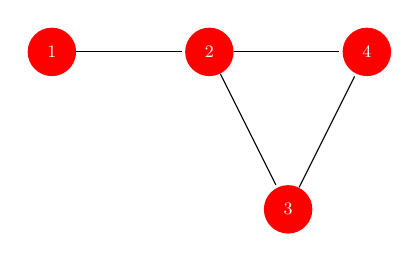
\begin{tikzpicture}
            \node[state] (1) at (0,0) {1}; 
            \node[state] (2) at (2,0) {2}; 
            \node[state] (3) at (3,-2) {3};
            \node[state] (4) at (4,0) {4};
            \onslide<3->{ \path (1) edge (2) ; }
            \onslide<4->{ \path (2) edge (3) (3) edge (4) (2) edge (4) ; }
          \end{tikzpicture}
        \end{center}
      \end{column}
    \end{columns}
  \end{block}

\end{frame}

\begin{frame}
  \frametitle{The Gaussian case}

  \begin{block}{The data}
    \begin{tikzpicture}
      \node[opacity=.75] at (-3,1.5) {\pgfuseimage{microarray}};
      \node[opacity=.9] at (-2.75,1.25) {\pgfuseimage{microarray}};
      \node[opacity=.95] at (-2.5,1) {\pgfuseimage{microarray}};
      \node at (-2.25,0.75) {\pgfuseimage{microarray}};
      \node[fill=red, text=white,single arrow] 
      (inference) at (0,1) {\sf \scriptsize Inference}; 
          
      \node at (4.5,1) {%
        $\mathbf{X} = \begin{pmatrix} 
          x_1^1 & x_1^2 & x_1^3 & \dots & x_1^p \\
          \vdots \\
          x_n^1 & x_n^2 & x_1^2 & \dots & x_n^p \\
        \end{pmatrix}$};
    \end{tikzpicture}
  \end{block}

  \begin{block}{Assuming $f_X(\mathbf{X})$ multivariate Gaussian}
    Greatly simplifies the inference:
    \begin{itemize}
    \item[$\rightsquigarrow$]   naturally   links   independence   and
      conditional   independence  to   the   covariance  and   partial
      covariance,
    \item[$\rightsquigarrow$]  gives a  straightforward interpretation
      to the graphical modeling previously considered.
  \end{itemize}
  \end{block}
\end{frame}


\begin{frame}
  \frametitle{Why Gaussianity helps?}
  \framesubtitle{Case of 2 variables or size-2 random vector}

  \begin{definitions}[Let $X,Y$ be two real random variables.]
    \vspace{-.75cm}
    \begin{equation*}
      \cov(X,Y)   =  \E\Big[\big(X-\E(X)\big)\big(Y-\E(Y)\big)\Big]  =
      \E(XY) - \E(X)\E(Y).
    \end{equation*}
    \begin{equation*}
      \rho_{XY} = \cor(X,Y) = \frac{\cov(X,Y)}{\sqrt{\var(X) \ \cdot \ \var(Y)}}.
    \end{equation*}
  \end{definitions}
  
  \begin{proposition}
    \begin{itemize}
    \item $\cov(X,X) = \var(X) = \E[(X-\E X)(Y-\E Y)]$,
    \item $\cov(X+Y,Z) = \cov(X,Z) + \cov(X,Z)$,
    \item $\var(X+Y) = \var(X) + \var(Y) + \cov(X,Y)$.
    \item $X \indep Y \Rightarrow\cov(X,Y) = 0$.
    \item<2> \alert{$X  \indep Y  \Leftrightarrow \cov(X,Y) =  0$ when
        $X,Y$ are Gaussian}.
    \end{itemize}
  \end{proposition}
\end{frame}

\begin{frame}
  \frametitle{The bivariate Gaussian distribution}

  \begin{columns}
    \begin{column}{.4\textwidth}
      \begin{block}{The Covariance Matrix}
        Let
        \begin{equation*}
          X \sim \mathcal{N}(\mathbf{0}, \boldsymbol\Sigma), 
        \end{equation*}
        with unit variance and $\rho_{XY} = \only<1>{0}\only<2>{0.9}$
        \begin{equation*}
          \boldsymbol\Sigma =
          \begin{pmatrix}
            1 & \only<1>{0}\only<2>{0.9} \\ \only<1>{0}\only<2>{0.9} & 1
          \end{pmatrix}.
        \end{equation*}
        The shape of the 2-D distribution evolves accordingly.
      \end{block}
    \end{column}
    
    \begin{column}{.6\textwidth}
      \includegraphics<1>[height=.8\textheight]{figures/multinorm_nocor}
      \includegraphics<2>[height=.8\textheight]{figures/multinorm_cor}
    \end{column}
  \end{columns}
\end{frame}

\begin{frame}
  \frametitle{Generalization: multivariate Gaussian vector}
  \framesubtitle{Now need partial covariance and partial correlation}
  
  Let $X,Y,Z$ be real random variables.
  \begin{definitions}
    \begin{equation*}
      \cov(X,Y|Z) = \cov(X,Y) - \cov(X,Z)\cov(Y,Z)/\var(Z).
    \end{equation*}
    \begin{equation*}
      \rho_{XY|Z}            =            \frac{\rho_{XY}            -
        \rho_{XZ}\rho_{YZ}}{\sqrt{1-\rho_{XZ}^2}\sqrt{1-\rho_{YZ}^2}}.
    \end{equation*}
  \end{definitions}
  $\rightsquigarrow$  Give   the  interaction  between   $X$  and  $Y$
  \alert{once removed the effect of $Z$}.

  \vfill
  
  \begin{proposition}<2>
    When $X,Y,Z$ are jointly Gaussian, then
    \begin{equation*}
      \alert{\cov(X,Y|Z) = 0  \Leftrightarrow \cor(X,Y|Z) = 0 \Leftrightarrow
      X \indep Y | Z.}
    \end{equation*}
  \end{proposition}
\end{frame}


\begin{frame}
  \frametitle{Gaussian Graphical Model: canonical settings}

  \begin{block}{Experiments in comparable Gaussian conditions}
    \begin{enumerate}
    \item  $X\sim\mathcal{N}(\boldsymbol\mu,\boldsymbol\Sigma)$,  with
      $\boldsymbol\Omega = \bSigma^{-1}$ the precision matrix.
    \item a sample $(X^1, \dots, X^n)$ of exp. stacked in an $n\times
      p$ data matrix $\mathbf{X}$.
    \end{enumerate}
  \end{block}

  \vspace{-.5cm}

  \begin{overlayarea}{\textwidth}{\textheight}
    \begin{block}{Conditional independence structure}
          \vspace{-.5cm}
          \begin{equation*}
            (i,j)  \notin  \mathcal{E}  \Leftrightarrow  X_i  \indep  X_j  |
            X_{\backslash \{i,j\}} \Leftrightarrow \Omega_{ij} = 0.
          \end{equation*}
        \end{block}
        
        \vspace{-.5cm}
        \begin{block}{Graphical interpretation}
          \vspace{-.5cm}
          \begin{center}
            \begin{tabular}{c@{\hspace{2cm}}c}
              \begin{tabular}{c}
                \small $\mathcal{G}=(\mathcal{P},\mathcal{E})$ \\
                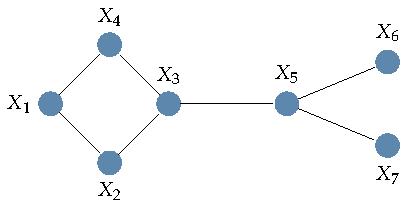
\includegraphics[width=.3\textwidth]{graph}
              \end{tabular}
              &
              \begin{tabular}{c}
                \small $\bTheta$\\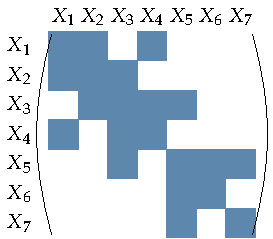
\includegraphics[width=.2\textwidth]{Markovadjacency}
              \end{tabular}
            \end{tabular}
          \end{center}
        \end{block}
        \vspace{-1cm}
        $\rightsquigarrow$ \alert{``Covariance'' selection}
   
  \end{overlayarea}      
\end{frame}

\begin{frame}
  \frametitle{Gaussian vector and linear regression (I)}

  \begin{proposition}[Gaussian vector and conditioning]
    \begin{equation*}
      Z = \begin{pmatrix}
        Z_1 \\ Z_2
      \end{pmatrix}  \sim   \mathcal{N}(\mathbf{0},\bSigma),   \quad
      \bSigma = \begin{pmatrix}
        \bSigma_{11} & \bSigma_{12} \\
        \bSigma_{21} & \bSigma_{22} \\
      \end{pmatrix},\quad
      \bOmega = \bSigma^{-1} = \begin{pmatrix}
        \bOmega_{11} & \bOmega_{12} \\
        \bOmega_{21} & \bOmega_{22} \\
      \end{pmatrix}.
    \end{equation*}
    Then,
    \begin{equation*}
      Z_2|Z_1=\mathbf{z} \sim
      \mathcal{N}\left(-\bOmega_{22}^{-1}\bOmega_{21}\mathbf{z}, \bOmega_{22}^{-1} \right)
    \end{equation*}
    and
    \begin{equation*}
      \bOmega_{22}^{-1}     =      \bSigma_{22}     -     \bSigma_{21}
      \bSigma_{11}^{-1} \bSigma_{12}.
    \end{equation*}
  \end{proposition}

  \vfill

  \begin{block}{Corollary}
    Partial correlations are related  to the inverse of the covariance
    matrix:
    \begin{equation*}
      \cor(Z_i,Z_j|Z_k, k\neq i,j) = - \frac{\Omega_{ij}}{\sqrt{\Omega_{ii}\Omega_{jj}}}
  \end{equation*}
  \end{block}

\end{frame}

\begin{frame}
  \frametitle{Gaussian vector and linear regression (II)}

  Consider the linear model
  \begin{equation}
      \label{eq:usual_lm}
    Y = X^\intercal\bbeta + \varepsilon, \quad \varepsilon\sim\mathcal{N}(0,\sigma).
  \end{equation}

  \begin{overlayarea}{\textwidth}{\textheight}

    \begin{block}{Other interpretation for the regression coefficients}
      If   $(X^T,  Y)^T\sim   \mathcal{N}(\mathbf{0},\bSigma)$  with   a
      block-wise  decomposion  of $\bSigma$  and  $\bOmega=\bSigma^{-1}$
      then by condition $Y|X$ we get
      \begin{equation}
        \label{eq:partial_lm}
        Y      =    \sum_{j=1}^p  X_j     \cor(X_j,Y|X_k,      k\neq      j)
        \sqrt{\frac{(\bOmega_{XX})_{jj}}{\omega_{YY}}}+ \varepsilon,
        \quad \varepsilon\sim\mathcal{N}(0,1/\omega_{YY}).
      \end{equation}

      By comparing \eqref{eq:usual_lm} to \eqref{eq:partial_lm}
      then \alert{$\beta_j$ is related to the partial correlation between $X_j$
        and $Y$},  i.e. describes  effect of  $X_j$ on  $Y$ once  effect of
      other predictors have been removed.
    \end{block}

  \end{overlayarea}
\end{frame}

\begin{frame}
  \frametitle{Gaussian Graphical Model and Linear Regression}

  \begin{block}{Linear regression viewpoint}
    Variable $X_i$ is linearly explained by the other variables:
    \begin{equation*}
      X_i | X_{ \setminus i} = - \sum_{j \neq i}
      \frac{\Theta_{ij}}{\Theta_{ii}} X_j + \varepsilon_i,\quad \varepsilon_i
      \sim \mathcal{N}(0,\sigma_i), \quad \varepsilon_i \perp X
      \end{equation*}
      Conditional  on its  neighborhood,  other variables do not  give
      additional insights
    \begin{equation*}
      X_i | X_{ \setminus i} = \sum_{\alert{j \in \text{neighbors}(i)}} \beta_j X_j + \varepsilon_i
      \quad         \text{with         }         \beta_j         =
      -\frac{\Theta_{ij}}{\Theta_{ii}}.
    \end{equation*}
  \end{block}

  % \vspace{-.5cm}
  % \begin{overlayarea}{\textwidth}{.45\textheight}
  %   \begin{block}{Graphical Interpretation}
  %     \vspace{-.5cm}
  %     \begin{center}
  %       \begin{scriptsize}
  %         \begin{tabular}{cc}
  %           Local Markov property & Global Markov property \\
  %           conditioning on the neighborhood & conditioning on a separating node\\
  %           \includegraphics[width=.4\textwidth]{localMarkov}
  %           & \includegraphics[width=.4\textwidth]{globalMarkov}\\
  %         \end{tabular}
  %       \end{scriptsize}
  %     \end{center}
  %   \end{block}
  % \end{overlayarea}

  \vfill
  \alert{$\rightsquigarrow$ ``Neighborhood'' selection}

\end{frame}


\section{Network Inference}

\pgfdeclareimage[height=0.8\textheight]{sparsity1}{figures/sparsity_1}
\pgfdeclareimage[height=0.8\textheight]{sparsity2}{figures/sparsity_2}
\pgfdeclareimage[height=0.375\textheight]{sparsity4}{figures/sparsity_4}

\begin{frame}
  \frametitle{References}

    \begin{thebibliography}{99}
      \setbeamertemplate{bibliography item}[book]

    \bibitem[JC]{JC} Habilitation, J. Chiquet, Chapter 2 \href{https://tel.archives-ouvertes.fr/tel-01288976/}{https://tel.archives-ouvertes.fr/tel-01288976/}
    \bibitem[EI]{EI} The Element of Statistical Learning \textcolor{black}{Hastie, Tibshirani, Friedman}, chapter 17.
    \end{thebibliography}

\end{frame}

\begin{frame}
  \frametitle{Some families of methods for network reconstruction}

  \begin{block}{Test-based methods}
    \vspace{-.15cm}
    \begin{itemize}
    \item Tests the nullity of each entries 
    \item Combinatorial problem when $p>30$ \dots
    \end{itemize}    
  \end{block}
  
  \vfill

  \begin{block}{Bayesian methods}
    \vspace{-.15cm}
    \begin{itemize}
    \item Compute the posterior probability of each edge
    \item Usually more computationally demanding
    \item For special graphs, computation gets easier
    \end{itemize}
  \end{block}

  \begin{block}{\alert{Sparsity-inducing regularization methods}}
    \vspace{-.15cm}
    \begin{itemize}
    \item induce sparsity with the $\ell_1$-norm penalization
    \item Use results from convex optimization
    \item Versatile and computationally efficient
    \end{itemize}
  \end{block}

\end{frame}

\subsection{Inducing sparsity for edge selection}

\begin{frame}
  \frametitle{Inference: maximum likelihood estimator}
  \framesubtitle{The natural approach for parametric statistics}

  Let   $X\sim f_{X}(x;\boldsymbol\Omega)$,  where   $\boldsymbol\Omega$  are  the
  model parameters.

  \vfill

  \begin{block}{Maximum likelihood estimator}
    \begin{equation*}
      \hat{\boldsymbol\Omega}      =      \argmax_{\boldsymbol\Omega}
      \ell(\boldsymbol\Omega; \mathbf{X})
    \end{equation*}
    where  $\ell$ is  the log  likelihood, a  function  of the
    parameters:
    \begin{equation*}
      \ell(\boldsymbol\Omega;      \mathbf{X})      =     \log
      \prod_{i=1}^n f_{X}(\mathbf{x}_i;\boldsymbol\Omega),
    \end{equation*}
    where $\mathbf{x}_i$ is the $i$th row of $\mathbf{X}$.
  \end{block}

  \vfill
  
  \begin{itemize}
    \item This a convex optimization problem,
    \item We just need to detect non zero coefficients in $\boldsymbol\Omega$
  \end{itemize}

\end{frame}

\begin{frame}
  \frametitle{The multivariate Gaussian log-likelihood }

  Let  $\mathbf{S}  =  n^{-1}\mathbf{X}^\intercal \mathbf{X}$  be  the
  empirical variance-covariance  matrix: $\mathbf{S}$ is  a sufficient
  statistic of $ \boldsymbol\Omega$.

  \vfill

  \begin{block}{The log-likelihood}
    \begin{equation*}
      \ell(\boldsymbol\Omega; \mathbf{S}) =
      \frac{n}{2}     \log    \det     (\boldsymbol\Omega)  - \frac{n}{2}
      \mathrm{Trace}(\mathbf{S} \boldsymbol\Omega) + \frac{n}{2}\log(2\pi).
    \end{equation*}
  \end{block}

  \vfill

  \begin{itemize}
  \item[$\rightsquigarrow$]    The     MLE    $=\mathbf{S}^{-1}$    of
    $\boldsymbol\Omega$ is not defined for $n< p$ and never sparse.
  \item[$\rightsquigarrow$] The need for regularization is huge.
  \end{itemize}
\end{frame}

\begin{frame}
  \frametitle{A Geometric View of Shrinkage}
  \framesubtitle{Constrained Optimization}

  \begin{overlayarea}{\textwidth}{\textheight}
    \begin{columns}
      \begin{column}{0.475\textwidth}
        \begin{tikzpicture}
          \only<1>{%
            \node (Surf) at (0,0) {\pgfuseimage{sparsity1}}
            node     at    (Surf.west)    [rotate=90,yshift=5mm]
            {$L(\Omega_1,\Omega_2;\mathbf{X})$}
            node at (Surf.south west) [xshift=5mm,yshift=5mm]{$\Omega_2$}
            node at (Surf.south east) [xshift=-7.5mm,yshift=2.5mm]{$\Omega_1$};
          }
          \only<2>{%
            \node (Surf2) at (0,0) {\pgfuseimage{sparsity2}}
            node    at    (Surf2.west)    [rotate=90,yshift=5mm]
            {$L(\Omega_1,\Omega_2;\mathbf{X})$}
            node at (Surf2.south west) [xshift=5mm,yshift=5mm]{$\Omega_2$}
            node at (Surf2.south east) [xshift=-7.5mm,yshift=2.5mm]{$\Omega_1$};
          }
          \only<3->{%
            \node (titi) at (0,0) {\phantom{titi}};
            \node (Surf3) at (0,-4.5) {\pgfuseimage{sparsity4}}
            node at (Surf3.west) [rotate=90,yshift=2.5mm] {$\Omega_2$}
            node at (Surf3.south) [yshift=-2.5mm] {$\Omega_1$};
          }
        \end{tikzpicture}
      \end{column}
      \begin{column}{0.55\textwidth}
        \only<1>{%
          We basically want to solve a problem of the form
          \begin{equation*}
            \maximize_{\Omega_1,\Omega_2} \ell(\Omega_1,\Omega_2;\mathbf{X})
          \end{equation*}
          where $\ell$ is typically a concave likelihood function.
        }
        \only<2->{%
          \begin{equation*}
            \left\{\begin{array}{ll}
                \displaystyle    \maximize_{\Omega_1,\Omega_2}   &
                \ell(\Omega_1,\Omega_2;\mathbf{X})\\
                \mathrm{s.t.} & \Omega(\Omega_1,\Omega_2) \leq c
              \end{array}\right.,
          \end{equation*}
          where  $\Omega$  defines  a  domain  that  \textit{constrains}
          $\boldsymbol\beta$.

          \begin{center}
            How shall we define $\Omega$ ?
          \end{center}
        }
      \end{column}
    \end{columns}
  \end{overlayarea}
\end{frame}


\pgfdeclareimage[height=0.375\textheight]{sparsity6}{figures/sparsity_6}
\pgfdeclareimage[height=0.375\textheight]{sparsity8bis}{figures/sparsity_8bis}
\pgfdeclareimage[height=0.375\textheight]{sparsity9}{figures/sparsity_9}
\pgfdeclareimage[height=0.375\textheight]{sparsity10}{figures/sparsity_10}
\pgfdeclareimage[height=0.375\textheight]{sparsity11}{figures/sparsity_11}
\pgfdeclareimage[height=0.375\textheight]{sparsity12}{figures/sparsity_12}


\begin{frame}
  \frametitle{A Geometric View of Sparsity}
  \framesubtitle{Dual and Polar Cones}

  {\centerline{Generalizes normals}}

  \bigskip

  \begin{overlayarea}{\textwidth}{\textheight}


    \begin{tikzpicture}
      \only<1>{%
      \node (Surf2) at (0,0) {\pgfuseimage{sparsity6}}
              node at (Surf2.west) [rotate=90,yshift=2.5mm] {$\beta_2$}
              node at (Surf2.south) [yshift=-1mm] {$\beta_1$};
      }
      \only<1-2>{%
      \node (Surf3) at (4,0) {\pgfuseimage{sparsity8bis}}
              node at (Surf3.west) [rotate=90,yshift=2.5mm] {$\beta_2$}
              node at (Surf3.south) [yshift=-1mm] {$\beta_1$};
      }
      \only<1-3>{%
        \node (Surf4) at (8,0) {\pgfuseimage{sparsity9}}
                node at (Surf4.west) [rotate=90,yshift=2.5mm] {$\beta_2$}
                node at (Surf4.south) [yshift=-1mm] {$\beta_1$};
      }
      \only<4>{%
        \node (Surf5) at (8,0) {\pgfuseimage{sparsity10}}
                node at (Surf5.west) [rotate=90,yshift=2.5mm] {$\beta_2$}
                node at (Surf5.south) [yshift=-1mm] {$\beta_1$};
      }
      \only<3->{%
        \node (Surf6) at (4,0) {\pgfuseimage{sparsity11}}
                node at (Surf6.west) [rotate=90,yshift=2.5mm] {$\beta_2$}
                node at (Surf6.south) [yshift=-1mm] {$\beta_1$};
      }
      \only<2->{%
        \node (Surf7) at (0,0) {\pgfuseimage{sparsity12}}
                node at (Surf7.west) [rotate=90,yshift=2.5mm] {$\beta_2$}
                node at (Surf7.south) [yshift=-1mm] {$\beta_1$};
      }
    \end{tikzpicture}

    \medskip

    Let $C$ be a convex set,
    \begin{itemize}
    \item  $C^\star(x_0) =  \set{y|y^T(x-x_0) \geq  0,x\in C}$  is the
      dual cone in $x_0$,
    \item $N_C(x_0) = \set{y|y^T(x-x_0) \leq 0,x\in C}$ is the polar (or normal) cone, 
    \end{itemize}

    \medskip

    \only<4>{%
      {\centerline{Shape of cones $\Rightarrow$ sparsity pattern}}
    }

  \end{overlayarea}
\end{frame}

\begin{frame}
  \frametitle{The Lasso}
  \framesubtitle{Least Absolute Shrinkage and Selection Operator}

  \begin{block}{Idea}
    Suggest  an admissible  set that  induces  \alert{sparsity} (force
    several entries to exactly zero in $\hat{\bbeta}$).
  \end{block}

  \vfill

  \begin{overlayarea}{\textwidth}{.4\textheight}
    \begin{columns}
      \begin{column}[c]{.6\textwidth}
        \begin{block}{Lasso as a regularization problem}
          The Lasso estimate of $\bbeta$ is the solution to
          \begin{equation*}
            \hat{\btheta}^{\text{lasso}}     =    \argmin_{\btheta}
            -\ell(\btheta),  \quad   \text{s.t.  }  \sum_{j=1}^p
            \left|\Omega_j\right|
            \leq s,
          \end{equation*}
          where $s$ is a shrinkage factor.
        \end{block}
      \end{column}
      \begin{column}{.4\textwidth}
        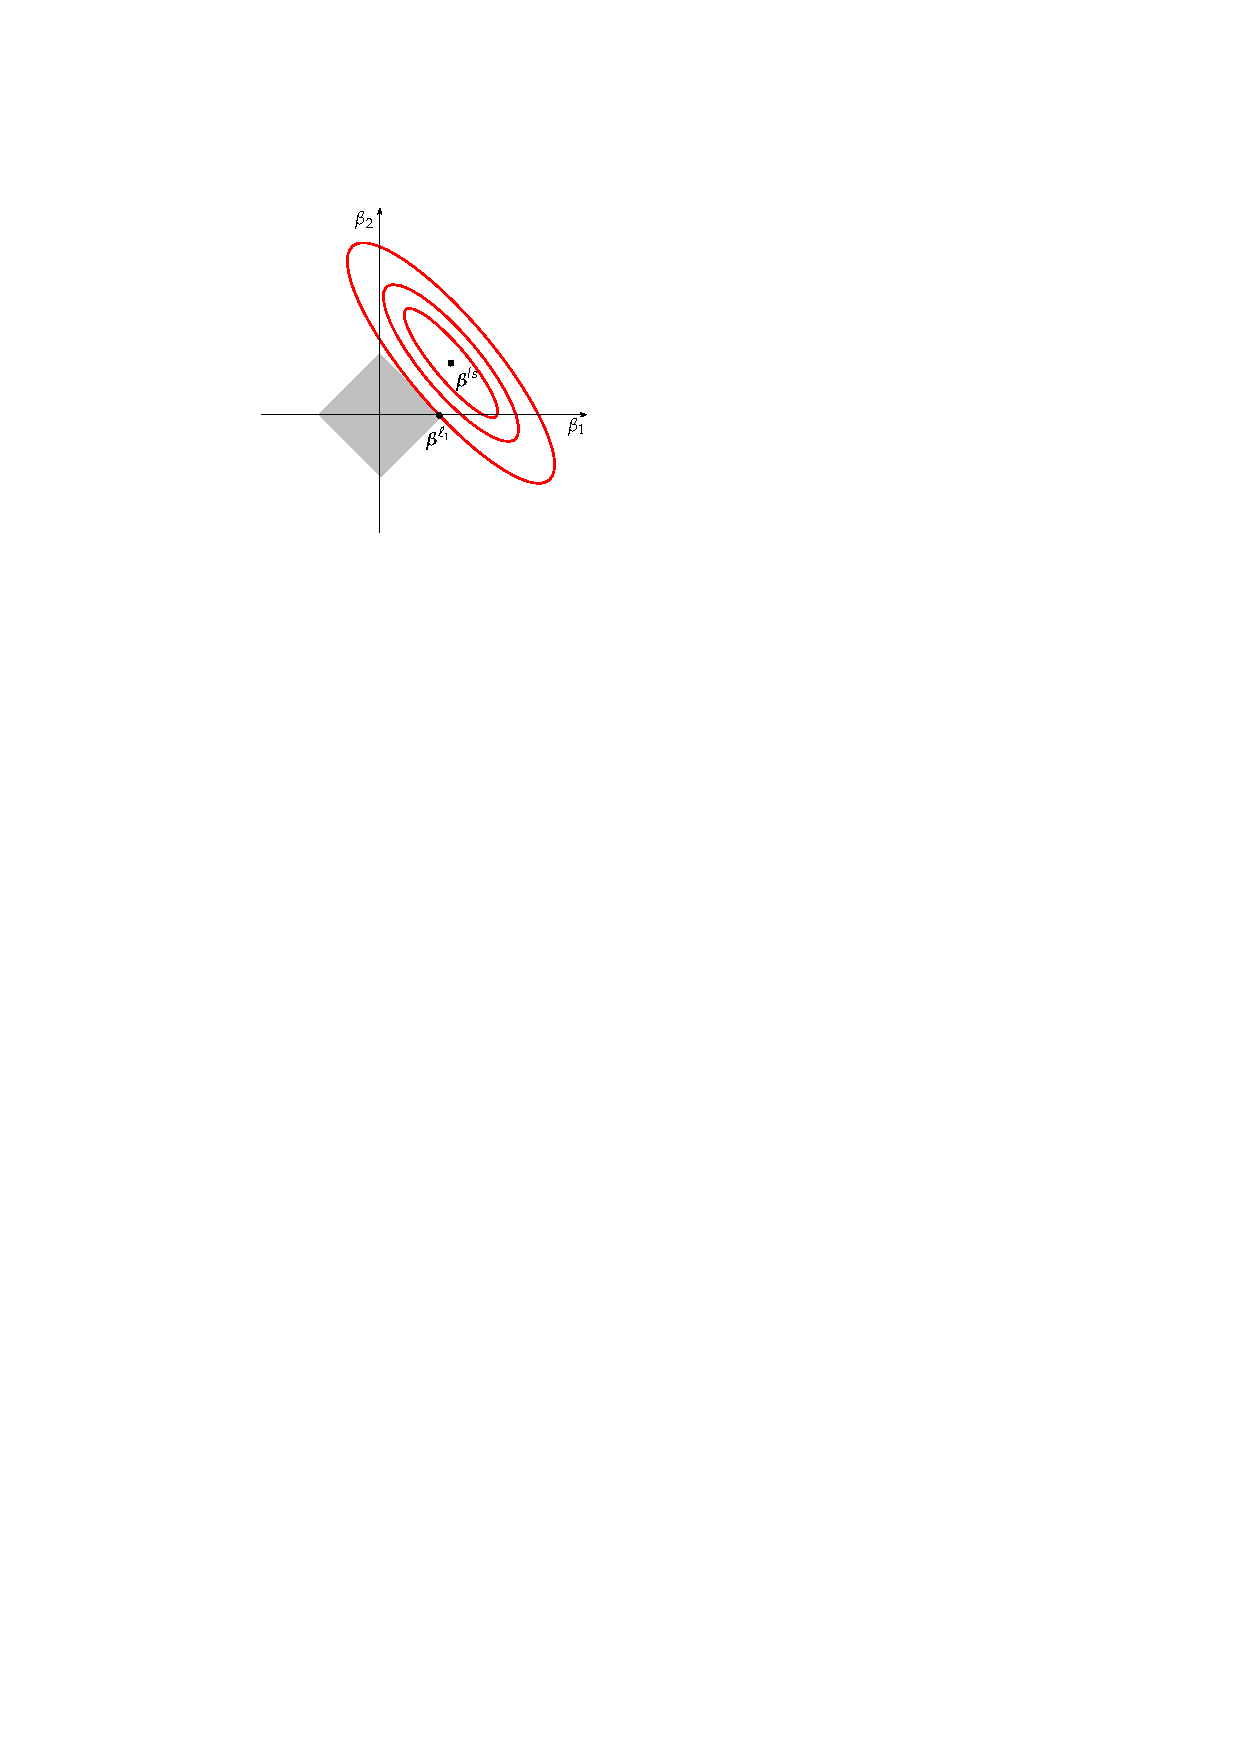
\includegraphics[width=.75\textwidth]{figures/lasso_set}
      \end{column}
    \end{columns}
  \end{overlayarea}

\end{frame}

\begin{frame}
  \frametitle{Insights: 2-dimensional example with the square loss}

  \begin{overlayarea}{\textwidth}{\textheight}

    \begin{equation*}
      \sum_{i=1}^n (y_i-x_i^1\Omega_1 - x_i^2\Omega_2)^2, \qquad
      \only<1>{\text{no constraints}}
      \only<2>{\text{s.t. } |\Omega_1| + |\Omega_2| < 0.75}
      \only<3>{\text{s.t. } |\Omega_1| + |\Omega_2| < 0.66}
      \only<4>{\text{s.t. } |\Omega_1| + |\Omega_2| < 0.4}
      \only<5>{\text{s.t. } |\Omega_1| + |\Omega_2| < 0.2}
      \only<6>{\text{s.t. } |\Omega_1| + |\Omega_2| < 0.0743}
    \end{equation*}

  \vspace{-.5cm}

    \includegraphics<1>[width=.8\textwidth]{dess11}
    \includegraphics<2>[width=.8\textwidth]{dess12}
    \includegraphics<3>[width=.8\textwidth]{dess13}
    \includegraphics<4>[width=.8\textwidth]{dess14}
    \includegraphics<5>[width=.8\textwidth]{dess15}
    \includegraphics<6>[width=.8\textwidth]{dess16}

  \end{overlayarea}

\end{frame}

\begin{frame}
  \frametitle{Application to GGM}

  \begin{block}{A penalized likelihood approach}
    \vspace{-1em}
    \begin{equation*}
      \hat{\bTheta}_\lambda=\argmax_{\bTheta \in \mathbb{S}_+}
      \ell(\bTheta;\mathbf{X})-\lambda
      \mathrm{pen}_{\ell_1}(\bTheta)
    \end{equation*}
  where
  \begin{itemize}
  \item $\mathcal{\ell}$ is the model log-likelihood,
  \item $\mathrm{pen}_{\ell_1}$ is a \alert{penalty function} tuned by
    $\lambda>0$.
    \vfill
      \begin{enumerate}
      \item \textit{regularization} (needed when $n \ll p$),
      \item \textit{selection} (sparsity induced by the $\ell_1$-norm).
      \end{enumerate}
  \end{itemize}
\end{block}

\end{frame}

\begin{frame}
  \frametitle{Gold standard penalized approaches}

  \vspace{-.25cm}
  
  \begin{overlayarea}{\textwidth}{\textheight}

    \begin{block}{Penalized   likelihood  (Banerjee   \textit{et
          al.}, Yuan and Lin, 2008)}
      \vspace{-1em}
      \begin{equation*}
        \hat{\bTheta}_\lambda=\argmax_{\bTheta \in \mathbb{S}_+}
        \ell(\bTheta;\mathbf{X})-\lambda
        \|\bTheta\|_{1}
      \end{equation*}
    \end{block}
    \vspace*{-1.5em}
    
    \begin{itemize}
    \item[\textcolor{green}{$+$}] symmetric, positive-definite
    \item[\textcolor{red}{$-$}]       solved      by       the
      ``Graphical-Lasso''                 ($\mathcal{O}(p^3)$,
      \textit{Friedman et al, 2007}).
    \item \texttt{R}-packages \textbf{glasso}, \textbf{quic}, \textbf{huge}.
    \end{itemize}
    
    \vfill
    
    \begin{block}{Neighborhood    Selection   (Meinshausen    \&
        B\"ulhman, 2006)}<2-> \vspace*{-1em}
      \only<2>{
         \begin{equation*}
          \text{For variable $j$, solve} \quad \hatbbeta_j  = \argmin_{\bbeta\in\Rset^{p-1}}
           \frac{1}{2} \|\bX_j - \bX_{\backslash j} \bbeta \|_2^2  + \lambda \|\bbeta\|_{\ell_1}.
          \end{equation*}
      }
      \only<3->{
      \begin{equation*}
        \hat{\mathbf{B}}^{\text{ns}}  = \argmin_{\mathbf{B}\in\Rset^{p\times  p}, \mathrm{diag}(\mathbf{B})
          = {\boldsymbol 0}_p} \frac{1}{2} \mathrm{tr}(\mathbf{B}^\top\mathbf{S}_n \mathbf{B}) -
        \mathrm{tr}(\mathbf{B}^\top\mathbf{S}_n) + \lambda \|\mathbf{B}\|_{\ell_1}.
      \end{equation*}
      }
      \vspace*{-1.5em}
    \end{block}
    
    \onslide<2->{
      \begin{itemize}
      \item[\textcolor{red}{$-$}]     not     symmetric,     not
        positive-definite
      \item[\textcolor{green}{$+$}]   $p$   Lasso  solved   with
        Lars-like   algorithms   ($\mathcal{O}(npd)$   for   $d$
        neighbors).
      \item \texttt{R}-package \textbf{huge}.
      \end{itemize}
    }
     
\end{overlayarea}      

\end{frame}

\subsection{Limitations and extensions of sparse GGM}

\begin{frame}
  \frametitle{Practical implications of theoretical results}

  \begin{block}{Selection    consistency    (Ravikumar,    Wainwright,
      2009-2012)}<1->                                           Denote
    $d=\max_{j\in\mathcal{P}}(\mathrm{degree_j})$.  Consistency for an
    appropriate $\lambda$ and
    \begin{itemize}
    \item  $n\approx\mathcal{O}(d^2\log(p))$ for  the graphical  Lasso
      and Clime.
    \item $n\approx\mathcal{O}(d\log(p))$  for   neighborhood
      selection (sharp).
    \end{itemize}
    \textit{(Irrepresentability) conditions are not strictly
    comparable\dots}
  \end{block}

  \vfill

  \begin{block}{Ultra high-dimension phenomenon (Verzelen,  2011)}<2>
    Minimax risk for sparse regression with $d$-sparse models: useless
    when
    \begin{equation*}
    \frac{d \log(p/d)}{n} \geq 1/2, \qquad (\mathrm{e.g.}, n=50, p=200, d\geq 8).
    \end{equation*}
    \textit{Good news! when $n$ is small, we don't need to solve
      huge problems because they can't but fail.}
  \end{block}

\end{frame}

\begin{frame}
  \frametitle{Model selection}

  \begin{block}{Cross-validation}
    Optimal in terms of \alert{prediction}, not in terms of selection
  \end{block}

  \begin{block}{Information based criteria}
    \begin{itemize}
    \item GGMSelect (Girault \textit{et al}, '12) selects among a family of candidates.
    \item Adapt IC to sparse high dimensional problems, e.g.
    \begin{equation*}
      \text{EBIC}_\gamma(\widehat{{\boldsymbol\Omega}}_\lambda)  =   -2 \textrm{loglik}
      (\widehat{{\boldsymbol\Omega}}_\lambda;\bX) + |\mathcal{E}_\lambda| (\log(n) + 4 \gamma \log(p) ),
    \end{equation*}
    \end{itemize}
  \end{block}

  \begin{block}{Resampling/subsampling}
    \alert{Keep edges frequently selected} on an range of $\lambda$ after sub-samplings
    \begin{itemize}
    \item Stability Selection (Meinshausen and B\"uhlman, 2010, Bach 2008)
    \item Stability approach to Regularization Selection (StaRS) (Liu, 2010).
    \end{itemize}
  \end{block}
\end{frame}

\subsection{Example: plasmodium data set}



\begin{frame}[fragile]
\frametitle{The plasmodium data}

\begin{knitrout}\scriptsize
\definecolor{shadecolor}{rgb}{0.969, 0.969, 0.969}\color{fgcolor}\begin{kframe}
\begin{alltt}
\hlkwd{library}\hlstd{(Matrix)}
\hlkwd{load}\hlstd{(}\hlstr{"plasmodium_expression.Rdata"}\hlstd{)}
\hlkwd{dim}\hlstd{(Y)}
\end{alltt}
\begin{verbatim}
## [1] 3490   46
\end{verbatim}
\begin{alltt}
\hlkwd{head}\hlstd{(Y)[,} \hlnum{1}\hlopt{:}\hlnum{5}\hlstd{]}
\end{alltt}
\begin{verbatim}
##                TP1    TP2    TP3    TP4    TP5
## MAL13P1.100 0.4510 0.6532 1.0760 0.5515 0.4238
## MAL13P1.102 1.5320 1.8920 0.8803 1.0300 0.9328
## MAL13P1.103 0.5218 0.5213 0.5328 0.3719 0.3258
## MAL13P1.105 0.5515 0.5527 0.8627 0.4541 0.4299
## MAL13P1.107 0.5630 0.4463 1.0760 0.4035 0.2082
## MAL13P1.112 0.5390 0.5393 0.5642 0.5326 0.4469
\end{verbatim}
\end{kframe}
\end{knitrout}
\end{frame}

\begin{frame}[fragile]
\frametitle{The plasmodium data}
\framesubtitle{Gene to Gene empirical covariance}

Covariance between the 100 most variable genes.

\begin{knitrout}\scriptsize
\definecolor{shadecolor}{rgb}{0.969, 0.969, 0.969}\color{fgcolor}\begin{kframe}
\begin{alltt}
\hlstd{genes.subset} \hlkwb{<-} \hlkwd{order}\hlstd{(}\hlkwd{apply}\hlstd{(Y,}\hlnum{1}\hlstd{,var))[}\hlnum{1}\hlopt{:}\hlnum{100}\hlstd{]}
\hlkwd{image}\hlstd{(}\hlkwd{Matrix}\hlstd{(}\hlkwd{cor}\hlstd{(}\hlkwd{t}\hlstd{(Y[genes.subset, ]))),} \hlkwc{userRaster}\hlstd{=}\hlnum{TRUE}\hlstd{)}
\end{alltt}
\end{kframe}
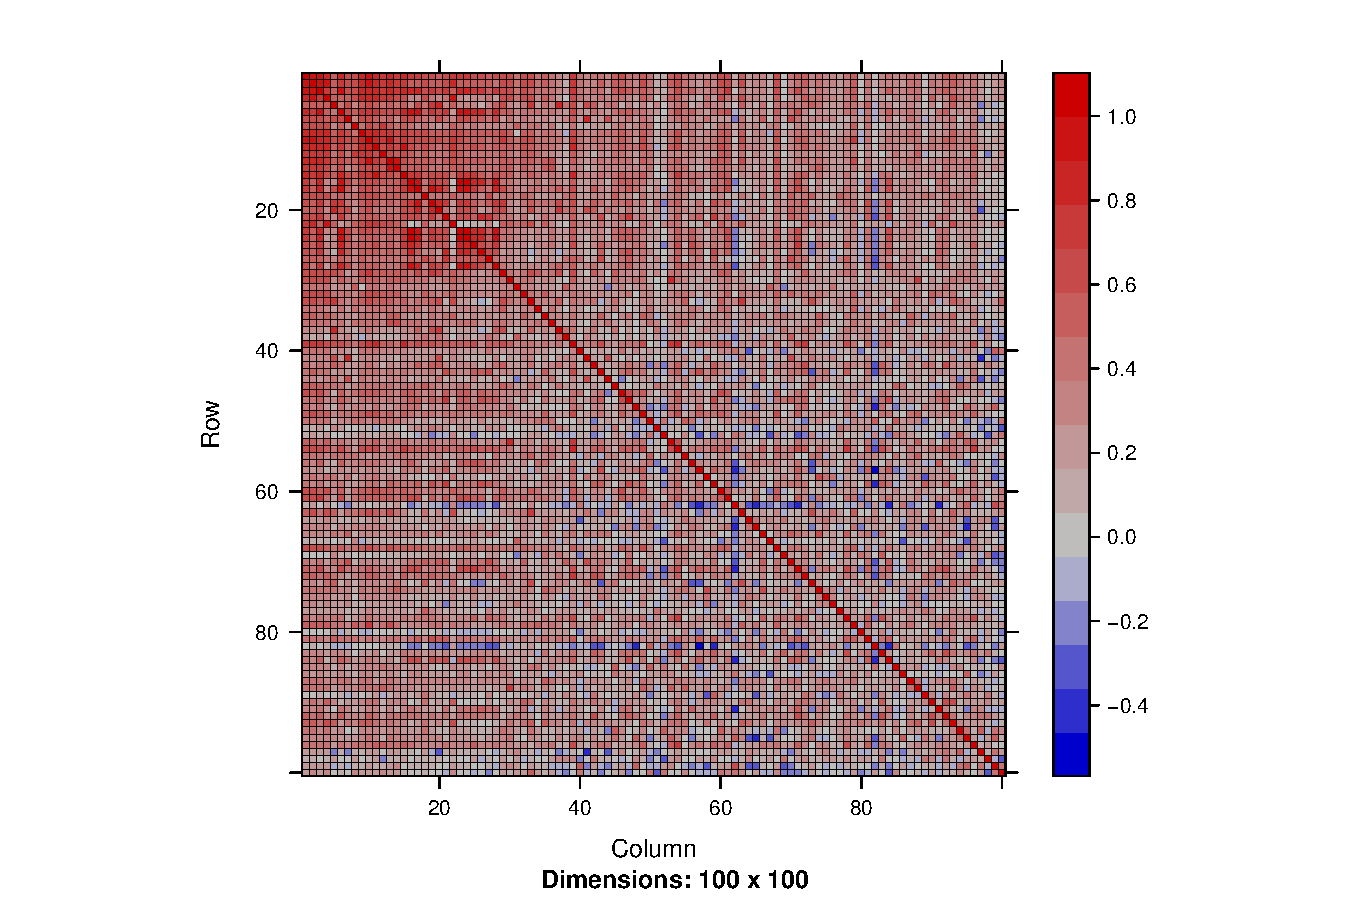
\includegraphics[width=.8\textwidth]{figures/get_plasmodium_data_fig-1} 

\end{knitrout}
\end{frame}

\begin{frame}[containsverbatim,allowframebreaks]
\frametitle{Network between the genes}
\framesubtitle{Sparse Estimation}

Regulatory network between the 100 most variable genes.

\begin{knitrout}\scriptsize
\definecolor{shadecolor}{rgb}{0.969, 0.969, 0.969}\color{fgcolor}\begin{kframe}
\begin{alltt}
\hlkwd{library}\hlstd{(huge)}
\hlstd{huge.out} \hlkwb{<-} \hlkwd{huge}\hlstd{(}\hlkwd{as.matrix}\hlstd{(}\hlkwd{t}\hlstd{(Y[genes.subset, ])),} \hlkwc{method}\hlstd{=}\hlstr{"glasso"}\hlstd{,} \hlkwc{cov.output}\hlstd{=}\hlnum{TRUE}\hlstd{)}
\end{alltt}
\begin{verbatim}
## Conducting the graphical lasso (glasso) with lossless screening....in progress:0% 
Conducting the graphical lasso (glasso) with lossless screening....in progress:9% 
Conducting the graphical lasso (glasso) with lossless screening....in progress:19% 
Conducting the graphical lasso (glasso) with lossless screening....in progress:30% 
Conducting the graphical lasso (glasso) with lossless screening....in progress:40% 
Conducting the graphical lasso (glasso) with lossless screening....in progress:50% 
Conducting the graphical lasso (glasso) with lossless screening....in progress:60% 
Conducting the graphical lasso (glasso) with lossless screening....in progress:70% 
Conducting the graphical lasso (glasso) with lossless screening....in progress:80% 
Conducting the graphical lasso (glasso)....done.                                          
\end{verbatim}
\begin{alltt}
\hlkwd{plot}\hlstd{(huge.out)}
\end{alltt}
\end{kframe}
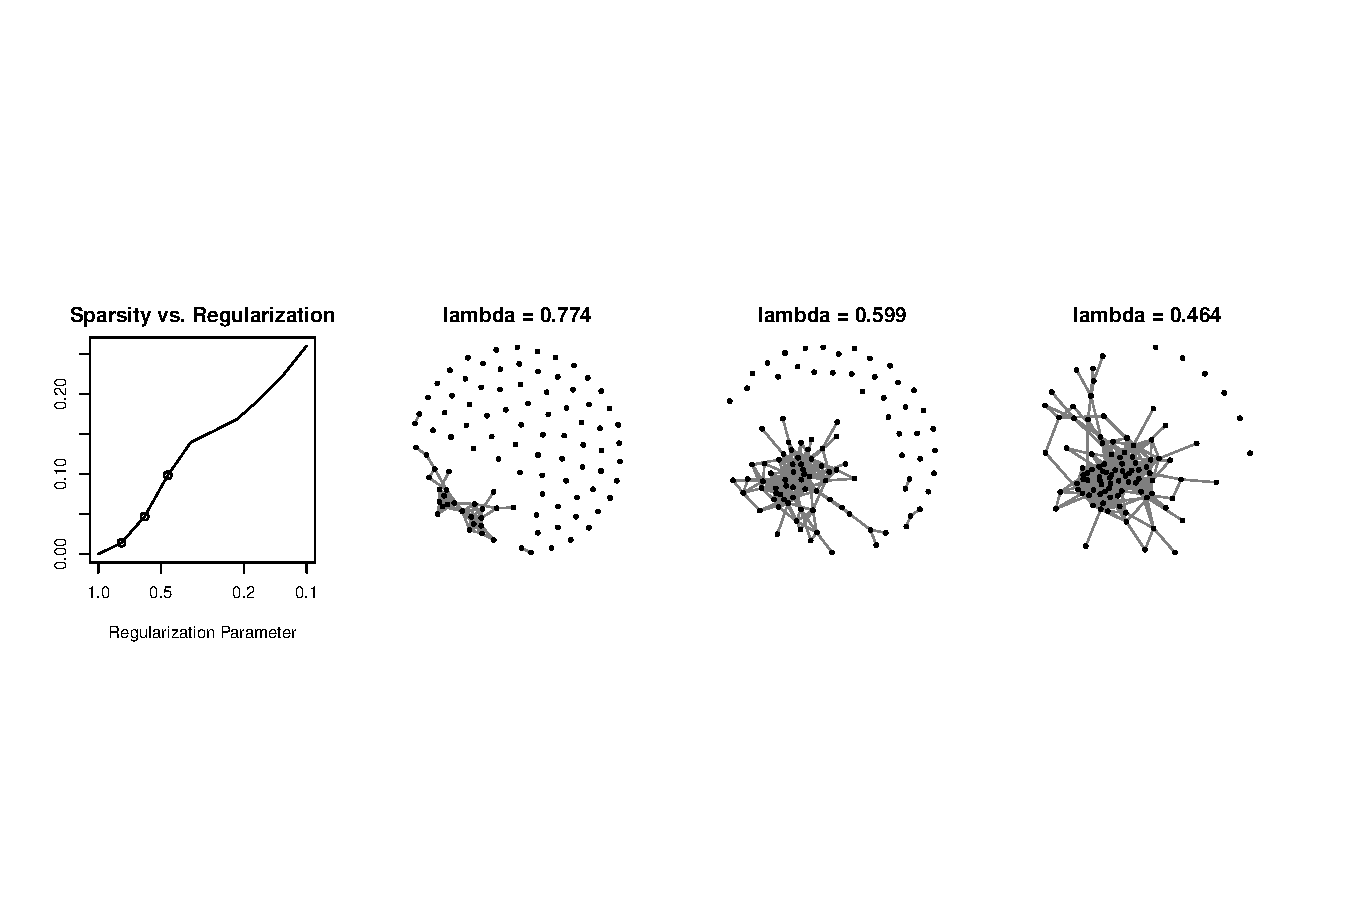
\includegraphics[width=.8\textwidth]{figures/r_show_plasmodium_glasso3-1} 

\end{knitrout}
\end{frame}

\begin{frame}[containsverbatim,allowframebreaks]
\frametitle{Network between the genes}
\framesubtitle{Inverse covariance}

\begin{knitrout}\scriptsize
\definecolor{shadecolor}{rgb}{0.969, 0.969, 0.969}\color{fgcolor}\begin{kframe}
\begin{alltt}
\hlkwd{library}\hlstd{(huge)}
\hlstd{huge.out}\hlopt{$}\hlstd{df}
\end{alltt}
\begin{verbatim}
##  [1]    0   71  233  488  693  763  836  963 1110 1289
\end{verbatim}
\begin{alltt}
\hlkwd{image}\hlstd{(}\hlkwd{Matrix}\hlstd{(huge.out}\hlopt{$}\hlstd{icov[[}\hlnum{3}\hlstd{]]))}
\end{alltt}
\end{kframe}
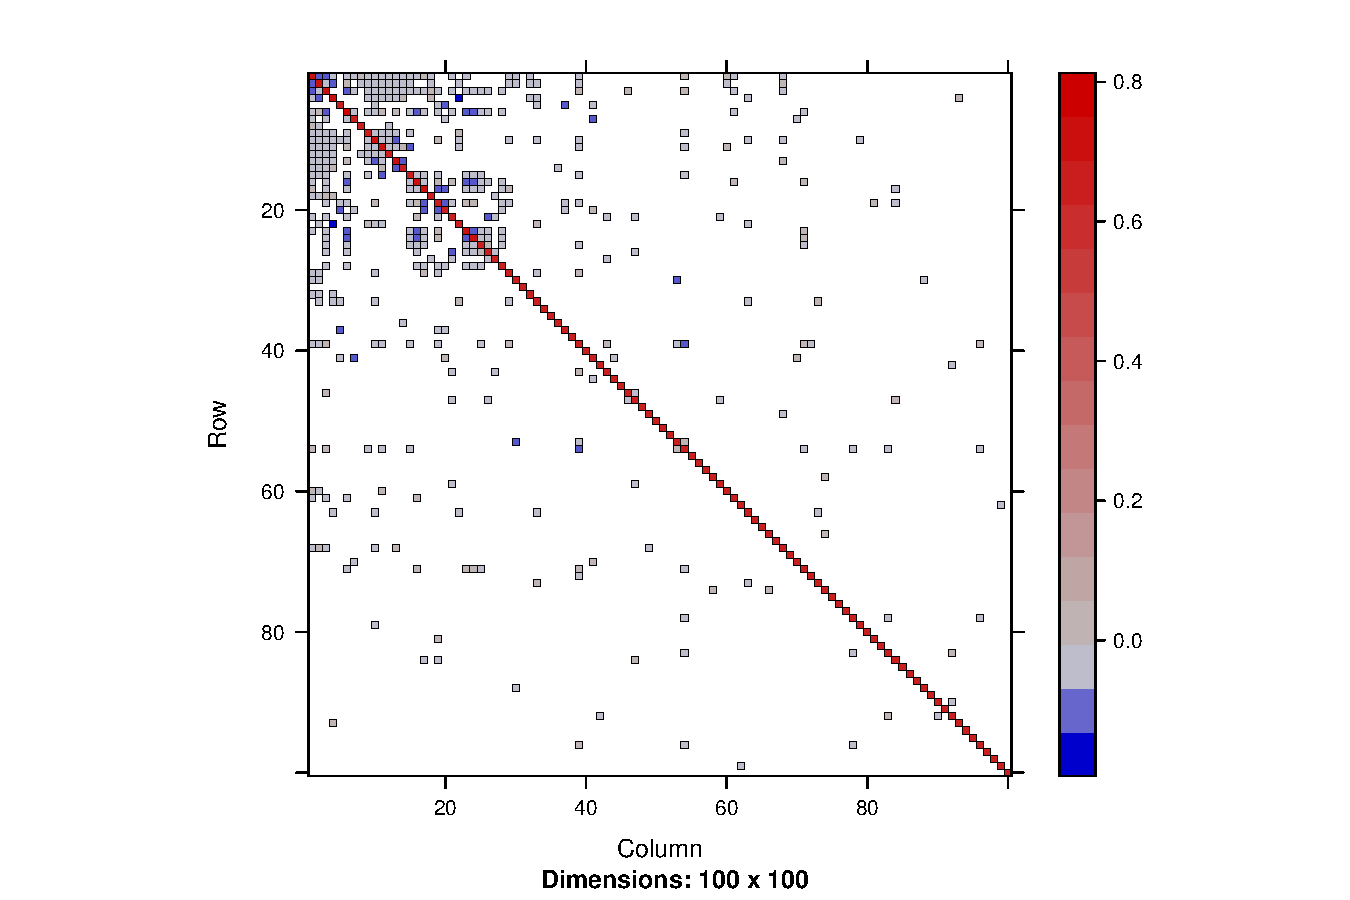
\includegraphics[width=.8\textwidth]{figures/r_show_plasmodium_glasso4-1} 

\end{knitrout}
\end{frame}

\begin{frame}[fragile]
\frametitle{The plasmodium data}
\framesubtitle{Covariance between conditions}

\begin{knitrout}\scriptsize
\definecolor{shadecolor}{rgb}{0.969, 0.969, 0.969}\color{fgcolor}\begin{kframe}
\begin{alltt}
\hlkwd{image}\hlstd{(}\hlkwd{Matrix}\hlstd{(}\hlkwd{cor}\hlstd{(Y)))}
\end{alltt}
\end{kframe}
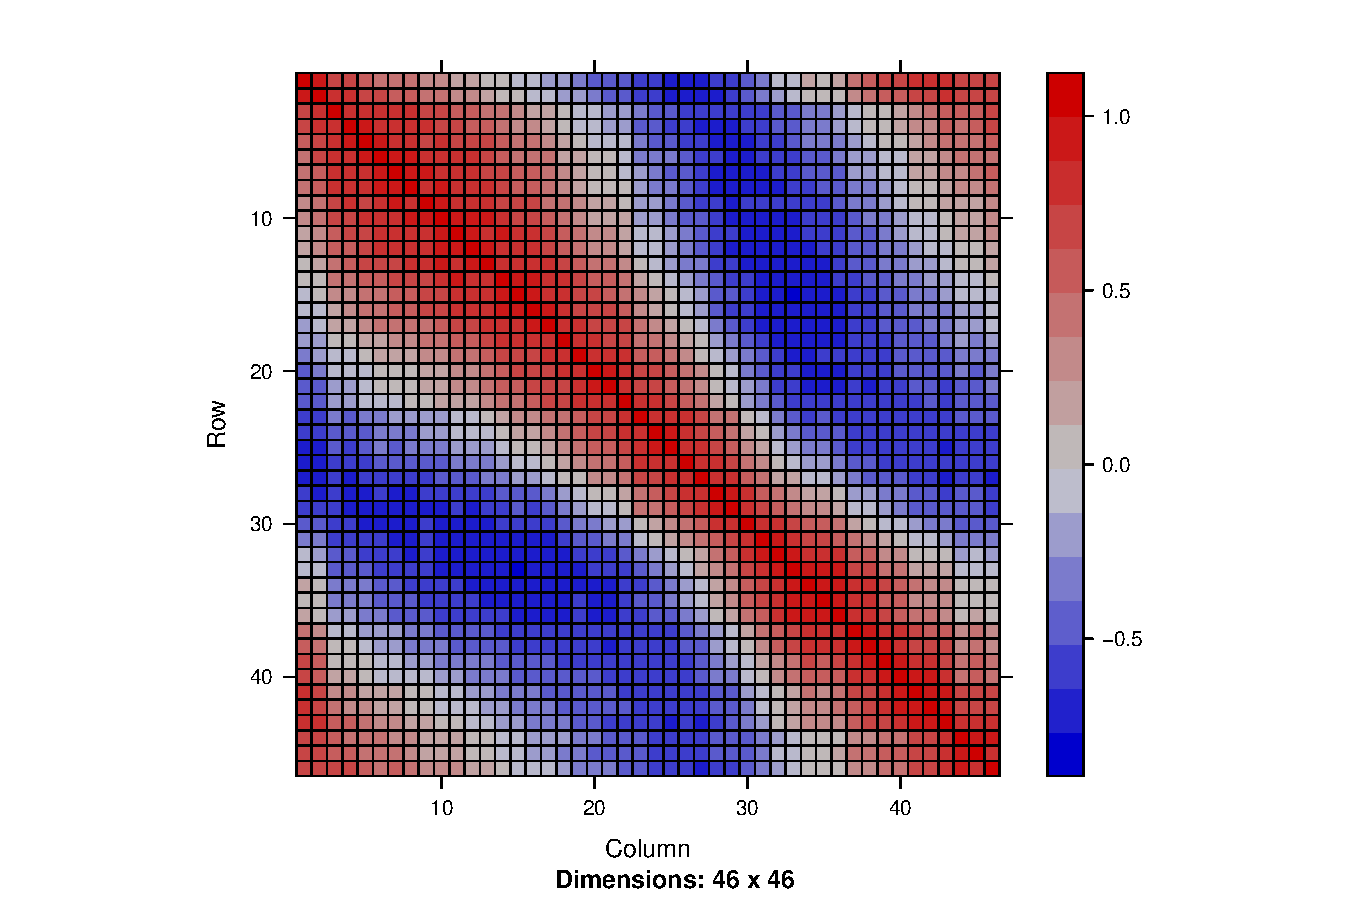
\includegraphics[width=.8\textwidth]{figures/get_plasmodium_data_fig_cond-1} 

\end{knitrout}
\end{frame}

\begin{frame}[containsverbatim]
\frametitle{Covariance structure between the conditions}
\framesubtitle{Sparse Estimation}

\begin{knitrout}\scriptsize
\definecolor{shadecolor}{rgb}{0.969, 0.969, 0.969}\color{fgcolor}\begin{kframe}
\begin{alltt}
\hlkwd{library}\hlstd{(huge)}
\hlstd{huge.out} \hlkwb{<-} \hlkwd{huge}\hlstd{(}\hlkwd{as.matrix}\hlstd{(Y),} \hlkwc{method}\hlstd{=}\hlstr{"glasso"}\hlstd{,} \hlkwc{cov.output}\hlstd{=}\hlnum{TRUE}\hlstd{)}
\end{alltt}
\begin{verbatim}
## Conducting the graphical lasso (glasso) with lossless screening....in progress:0% 
Conducting the graphical lasso (glasso) with lossless screening....in progress:9% 
Conducting the graphical lasso (glasso) with lossless screening....in progress:19% 
Conducting the graphical lasso (glasso) with lossless screening....in progress:30% 
Conducting the graphical lasso (glasso) with lossless screening....in progress:40% 
Conducting the graphical lasso (glasso) with lossless screening....in progress:50% 
Conducting the graphical lasso (glasso) with lossless screening....in progress:60% 
Conducting the graphical lasso (glasso) with lossless screening....in progress:70% 
Conducting the graphical lasso (glasso) with lossless screening....in progress:80% 
Conducting the graphical lasso (glasso)....done.                                          
\end{verbatim}
\begin{alltt}
\hlstd{sel.out}  \hlkwb{<-} \hlkwd{huge.select}\hlstd{(huge.out)}
\end{alltt}
\begin{verbatim}
## Conducting extended Bayesian information criterion (ebic) selection....done
\end{verbatim}
\end{kframe}
\end{knitrout}
\end{frame}

\begin{frame}[containsverbatim]
\frametitle{Covariance structure between the conditions}
\framesubtitle{Sparse Estimation}

\begin{knitrout}\scriptsize
\definecolor{shadecolor}{rgb}{0.969, 0.969, 0.969}\color{fgcolor}\begin{kframe}
\begin{alltt}
\hlkwd{image}\hlstd{(sel.out}\hlopt{$}\hlstd{opt.cov)}
\end{alltt}
\end{kframe}
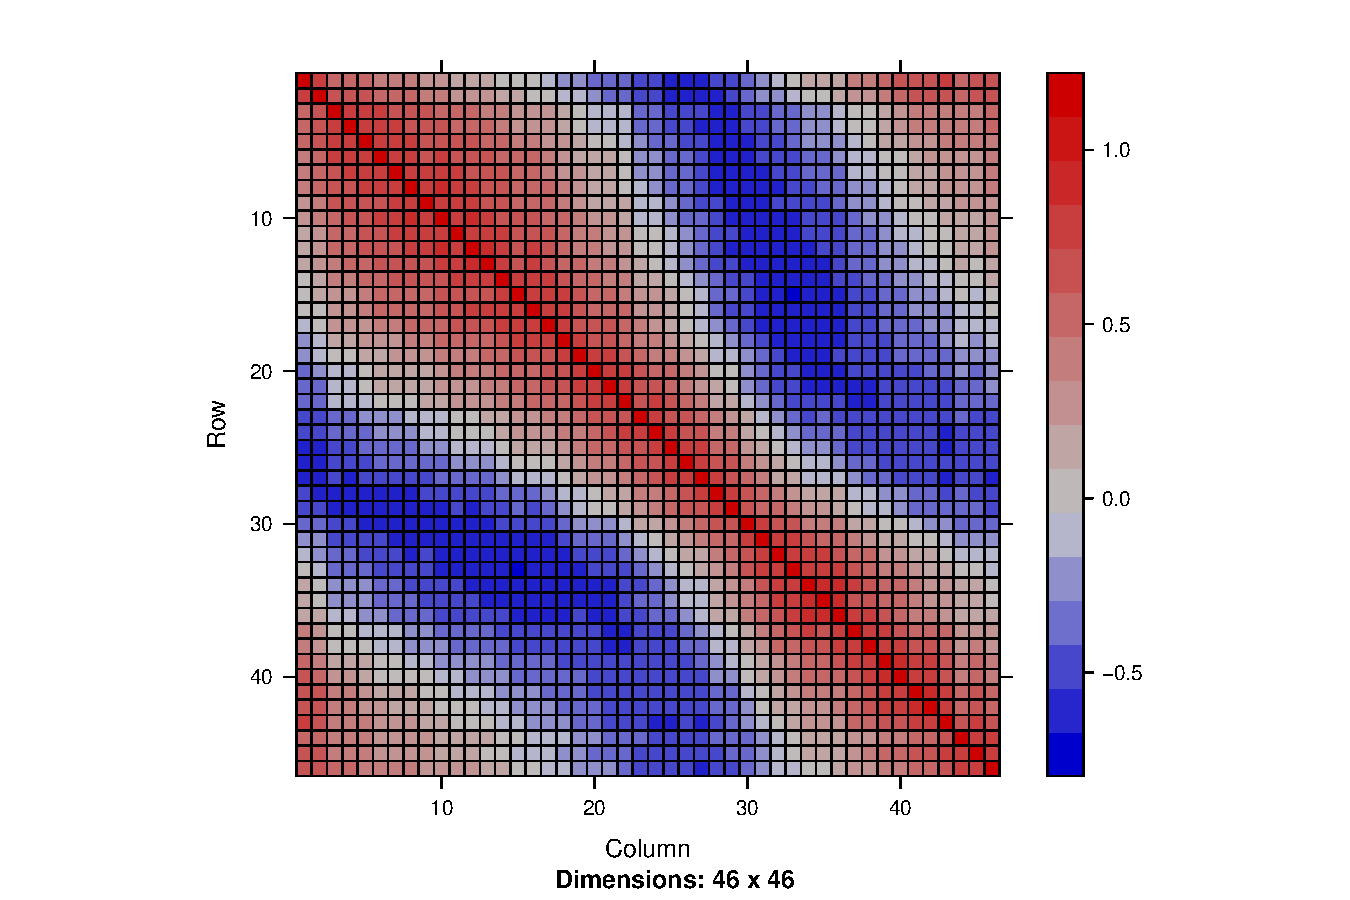
\includegraphics[width=.8\textwidth]{figures/r_get_plasmodium_glassob-1} 

\end{knitrout}
\end{frame}

\begin{frame}[containsverbatim,allowframebreaks]
\frametitle{Covariance structure between the conditions}
\framesubtitle{Sparse Estimation of the inverse covariance}

\begin{knitrout}\scriptsize
\definecolor{shadecolor}{rgb}{0.969, 0.969, 0.969}\color{fgcolor}\begin{kframe}
\begin{alltt}
\hlkwd{sum}\hlstd{(}\hlkwd{abs}\hlstd{(sel.out}\hlopt{$}\hlstd{opt.icov)} \hlopt{!=} \hlnum{0}\hlstd{)}
\end{alltt}
\begin{verbatim}
## [1] 760
\end{verbatim}
\begin{alltt}
\hlkwd{ncol}\hlstd{(sel.out}\hlopt{$}\hlstd{opt.icov)} \hlopt{**} \hlnum{2}
\end{alltt}
\begin{verbatim}
## [1] 2116
\end{verbatim}
\begin{alltt}
\hlkwd{image}\hlstd{(sel.out}\hlopt{$}\hlstd{opt.icov)}
\end{alltt}
\end{kframe}
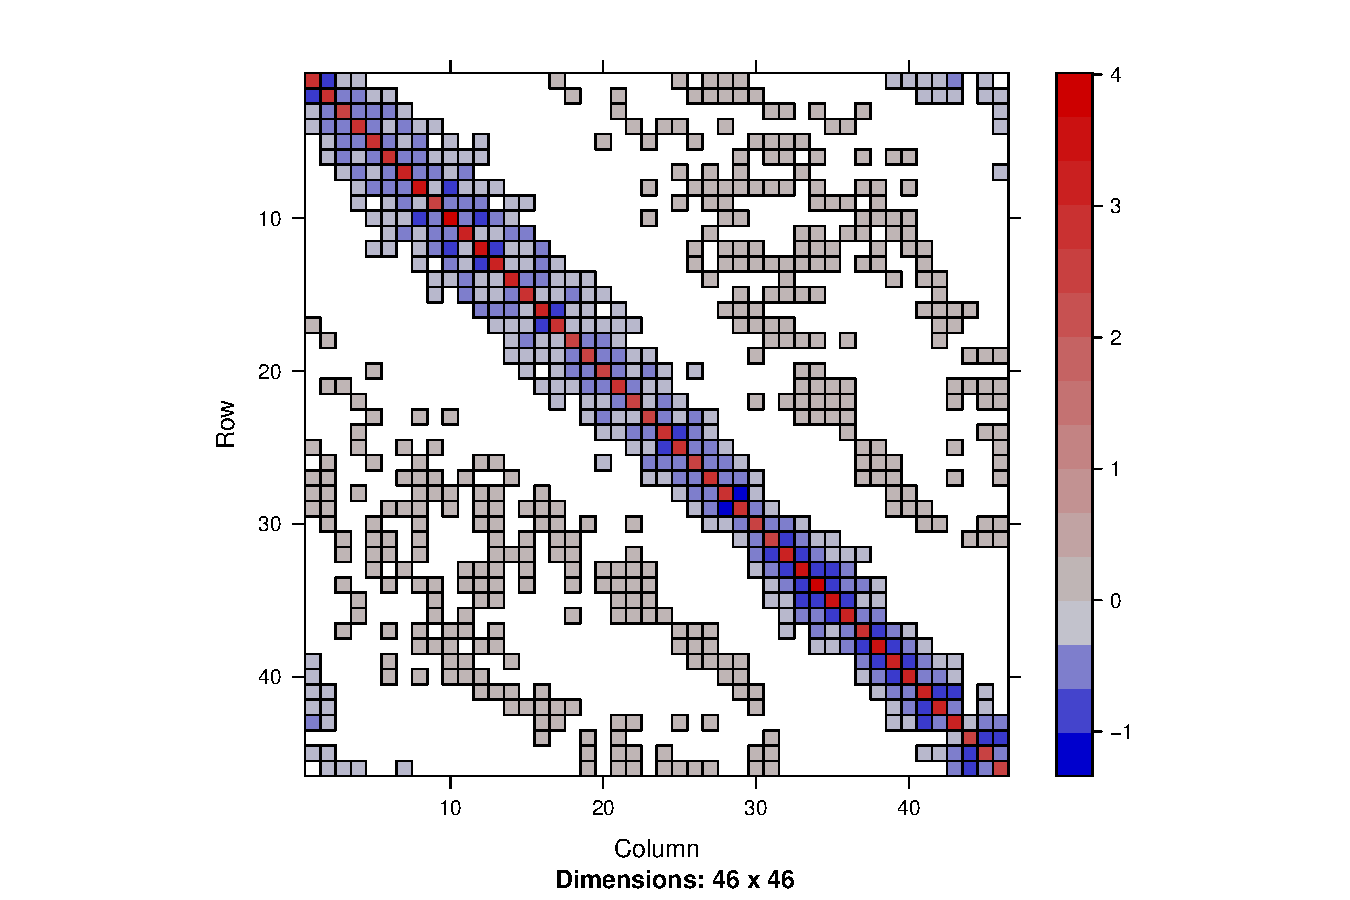
\includegraphics[width=.8\textwidth]{figures/r_show_plasmodium_glasso-1} 

\end{knitrout}

\end{frame}

\begin{frame}[containsverbatim,allowframebreaks]
\frametitle{Covariance structure between the conditions}
\framesubtitle{Associated network}

\begin{knitrout}\scriptsize
\definecolor{shadecolor}{rgb}{0.969, 0.969, 0.969}\color{fgcolor}\begin{kframe}
\begin{alltt}
\hlkwd{plot}\hlstd{(huge.out)}
\end{alltt}
\end{kframe}
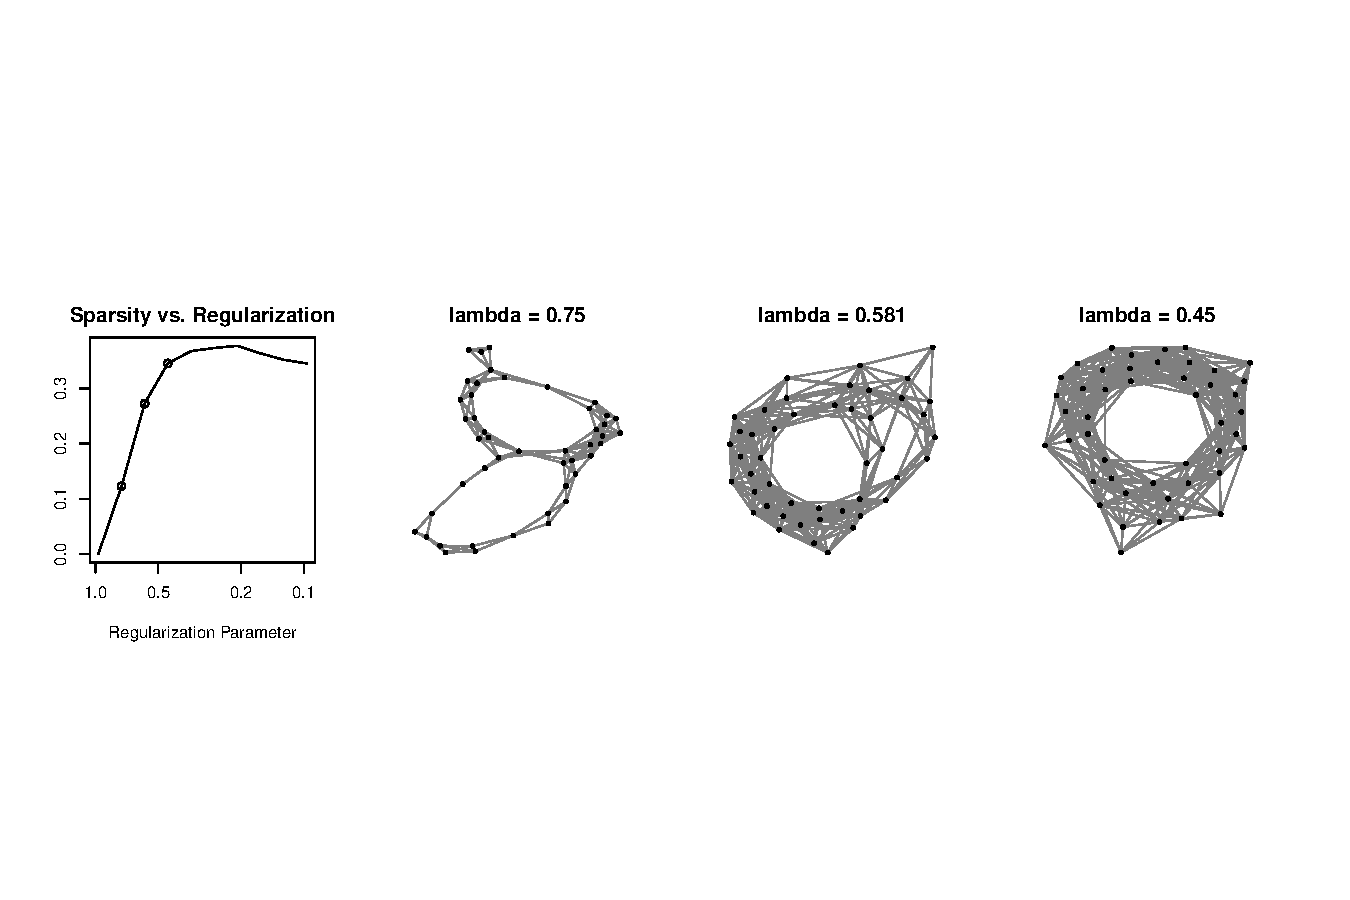
\includegraphics[width=.8\textwidth]{figures/r_show_plasmodium_glasso2-1} 

\end{knitrout}

\end{frame}




\end{document}
